\documentclass[10pt]{book}

%These tell TeX which packages to use.
\usepackage{array,epsfig}
\usepackage{amsmath}
\usepackage{amsfonts}
\usepackage{amssymb}
\usepackage{amsxtra}
\usepackage{amsthm}
\usepackage{mathrsfs}
\usepackage{color}
\usepackage{enumitem}
\usepackage{wrapfig}
\usepackage{pgfplots}
\pgfplotsset{compat=1.6}

\pgfplotsset{soldot/.style={color=black,only marks,mark=*}} \pgfplotsset{holdot/.style={color=black,fill=white,only marks,mark=*}}

%Here I define some theorem styles and shortcut commands for symbols I use often
\theoremstyle{definition}
\newtheorem{defn}{Definition}
\newtheorem{thm}{Theorem}
\newtheorem{cor}{Corollary}
\newtheorem*{rmk}{Remark}
\newtheorem{lem}{Lemma}
\newtheorem*{joke}{Joke}
\newtheorem{ex}{Example}
\newtheorem*{soln}{Solution}
\newtheorem{prop}{Proposition}

\newcommand{\lra}{\longrightarrow}
\newcommand{\ra}{\rightarrow}
\newcommand{\surj}{\twoheadrightarrow}
\newcommand{\graph}{\mathrm{graph}}
\newcommand{\bb}[1]{\mathbb{#1}}
\newcommand{\Z}{\bb{Z}}
\newcommand{\Q}{\bb{Q}}
\newcommand{\R}{\bb{R}}
\newcommand{\C}{\bb{C}}
\newcommand{\N}{\bb{N}}
\newcommand{\M}{\mathbf{M}}
\newcommand{\m}{\mathbf{m}}
\newcommand{\MM}{\mathscr{M}}
\newcommand{\HH}{\mathscr{H}}
\newcommand{\Om}{\Omega}
\newcommand{\Ho}{\in\HH(\Om)}
\newcommand{\bd}{\partial}
\newcommand{\del}{\partial}
\newcommand{\bardel}{\overline\partial}
\newcommand{\textdf}[1]{\textbf{\textsf{#1}}\index{#1}}
\newcommand{\img}{\mathrm{img}}
\newcommand{\ip}[2]{\left\langle{#1},{#2}\right\rangle}
\newcommand{\inter}[1]{\mathrm{int}{#1}}
\newcommand{\exter}[1]{\mathrm{ext}{#1}}
\newcommand{\cl}[1]{\mathrm{cl}{#1}}
\newcommand{\ds}{\displaystyle}
\newcommand{\vol}{\mathrm{vol}}
\newcommand{\cnt}{\mathrm{ct}}
\newcommand{\osc}{\mathrm{osc}}
\newcommand{\LL}{\mathbf{L}}
\newcommand{\UU}{\mathbf{U}}
\newcommand{\support}{\mathrm{support}}
\newcommand{\AND}{\;\wedge\;}
\newcommand{\OR}{\;\vee\;}
\newcommand{\Oset}{\varnothing}
\newcommand{\st}{\ni}
\newcommand{\wh}{\widehat}
%Pagination stuff.
\setlength{\topmargin}{-0.75in}
\setlength{\oddsidemargin}{0in}
\setlength{\evensidemargin}{0in}
\setlength{\textheight}{9.in}
\setlength{\textwidth}{6.5in}
\pagestyle{empty}
\begin{document}
\begin{flushleft}
Name:\underline{\hspace{13cm}}Date:\underline{\hspace{2cm}}
\end{flushleft}
\begin{center}
{\Large \hspace{0.5cm} Quiz \#9 Makeup/Replacement Quiz, Due Friday 3-27 by 11:59pm}
\end{center}
\vspace{0.2 cm}
\subsection*{Problem 1} 
On the grid below, sketch the graph of a function $f(x)$ with domain $[-6,5]$ that has the given properties:
\\
\begin{wrapfigure}{l}{0.4\textwidth}
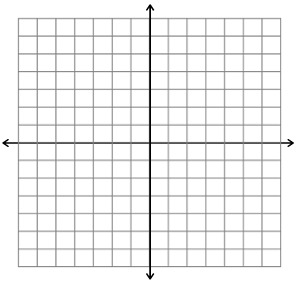
\includegraphics[width=\linewidth]{blankgrid1.jpg} 
 \vspace{-110pt}
\end{wrapfigure}
\begin{itemize}
    \item Absolute maximum at $x=-6$,
    \item Absolute minimum at $x=2$,
    \item Local maximum at $x=0$,
    \item $\displaystyle\lim_{x\rightarrow 5^-}f(x)=f(5)=0$,
    \item $\displaystyle\lim_{x\rightarrow -2^-}f(x)=2$.
    \item $\displaystyle\lim_{x\rightarrow -2^+}f(x)=1$
    \item Right continuous at $x=-2$.
    \item $\displaystyle\lim_{x\rightarrow 3}f(x)=1$, with a removable discontinuity.
    \item $f(3)=0$.
\end{itemize}
\vspace{1cm}
\subsection*{Problem 2} A spherical balloon's volume is increasing at a rate of $\displaystyle 8\pi$ cubic inches per second when the radius is one inch. How fast is the surface area of the balloon increasing when the radius is one inch?
\clearpage
\subsection*{Problem 3} The position of a quantum particle is given by 
\[
s(t)=2t(t^2-6t+9),
\]
where $s$ is in nanometers, and $t$ is in seconds.
\begin{enumerate}[label=(\alph*)]
    \item When is the particle at rest?\vspace{2cm}
    \item When does the particle move forward?\vspace{2cm}
    \item When does the particle move backward?\vspace{2cm}
    \item When does the particle change direction?\vspace{2cm}
    \item What is the total distance traveled by the particle after six seconds?\vspace{3cm}
    \item When is the particle accelerating? When is it decelerating?\vspace{2cm}
\end{enumerate}
\clearpage
\subsection*{Problem 4} The height (in meters) of a projectile shot vertically upward from a point ten meters above ground level with an initial velocity of 49 meters per second is given by $10+49t-4.9t^2$ after $t$ seconds.
\begin{enumerate}[label=(\alph*)]
    \item Find the velocity after 2 seconds and 4 seconds.\vspace{2cm}
    \item When does the projectile reach maximum height?\vspace{2cm}
    \item What is the maximum height?\vspace{2cm}
    \item When does it hit the ground and with what velocity does it hit the ground?\vspace{3cm}
\end{enumerate}
\subsection*{Problem 5} Calculate $y'$. Show work, no work = no credit!
\begin{enumerate}[label=(\alph*)]
    \item $\displaystyle y=(x^2+x^4)^5$\vspace{3cm}
    \item $\displaystyle y=\frac{e^{1/y}}{x^2}$\vspace{3cm}
\end{enumerate}
%(Problem 5 Continued\ldots)
%\begin{enumerate}[resume,label=(\alph*)]
%    \item $\displaystyle y=\sin\left(\arctan\sqrt{1+x^2}\right)$\vspace{3cm}
%    \item $xe^y=y^2-x^2$\vspace{4cm}
%\end{enumerate}
%\subsection*{Problem 6} Find the absolute maximum and absolute minimum values of $\displaystyle f(x)=2\cos x+\sin 2x$ on the interval $[0,\pi/2]$.
\end{document}